\documentclass[11pt]{article}


\usepackage{fullpage}
\usepackage{graphicx}
\usepackage{amsmath}
\usepackage{amssymb}
\usepackage{amsthm}
\usepackage{fancyvrb}

\newcommand{\myname}{Mehshan Mustafa}

\newenvironment{theorem}[2][Theorem]{\begin{trivlist}
\item[\hskip \labelsep {\bfseries #1}\hskip \labelsep {\bfseries #2.}]}{\end{trivlist}}
\newenvironment{lemma}[2][Lemma]{\begin{trivlist}
\item[\hskip \labelsep {\bfseries #1}\hskip \labelsep {\bfseries #2.}]}{\end{trivlist}}
\newenvironment{exercise}[2][Exercise]{\begin{trivlist}
\item[\hskip \labelsep {\bfseries #1}\hskip \labelsep {\bfseries #2.}]}{\end{trivlist}}
\newenvironment{problem}[2][Problem]{\begin{trivlist}
\item[\hskip \labelsep {\bfseries #1}\hskip \labelsep {\bfseries #2.}]}{\end{trivlist}}
\newenvironment{question}[2][Question]{\begin{trivlist}
\item[\hskip \labelsep {\bfseries #1}\hskip \labelsep {\bfseries #2.}]}{\end{trivlist}}
\newenvironment{corollary}[2][Corollary]{\begin{trivlist}
\item[\hskip \labelsep {\bfseries #1}\hskip \labelsep {\bfseries #2.}]}{\end{trivlist}}
\newenvironment{solution}{\begin{proof}[Solution]}{\end{proof}}
\newenvironment{idea}[2][Proof Idea.]{\textit{#1} #2}



\parindent0in
\pagestyle{plain}
\thispagestyle{plain}

\newcommand{\dated}{\today}
\newcommand{\token}[1]{\langle \text{#1} \rangle}

\begin{document}

\textbf{Introduction to the Theory of
Computation}\hfill\textbf{\myname}\\[0.01in]
\textbf{Chapter 3: The Church-Turing Thesis}\hfill\textbf{\dated}\\
\smallskip\hrule\bigskip

\begin{problem}{3.14}
A \textbf{\textit{queue automaton}} is like a push-down automaton except that the stack is replaced by a queue. A \textbf{\textit{queue}} is a tape allowing symbols to be written only on the left-hand end and read only at the right-hand end. Each write operation (we’ll call it a \textit{push}) adds a symbol to the left-hand end of the queue and each read operation (we'll call it a \textit{pull}) reads and removes a symbol at the right-hand end. As with a PDA, the input is placed on a separate read-only input tape, and the head on the input tape can move only from left to right. The input tape contains a cell with a blank symbol following the input, so that the end of the input can be detected. A queue automaton accepts its input by entering a special accept state at any time. Show that a language can be recognized by a deterministic queue automaton iff the language is Turing-recognizable.
\end{problem}

\begin{proof}
To show that a language can be recognized by a deterministic queue automaton iff the language is Turing-recognizable, we show that queue automata and Turing machines are equivalent. \\
\\
First we show how a Turing machine can simulate any queue automaton.
\begin{enumerate}
\item Use two tapes, an input tape that contains the input string and a second tape for the queue (we call it the \textit{queue tape}).
\item To push a symbol, write the symbol on the first blank cell on the queue tape.
\item To pull, find the first uncrossed symbol on the queue tape. Read the symbol and mark it as crossed. If there is no such symbol, then it means that the queue is empty.
\end{enumerate}
Next, we show how a queue automaton can simulate Turing machines. The queue is used to simulate Turing machine tape, and the move left and right operations. At the start, load the queue with input string. Two special symbols are used.
\begin{enumerate}
\item Hash symbol $\#$ is used to mark the end of the input string. It is also used to mark the beginning of infinite tape.
\item Dollar symbol $\$$ marks the end of the queue.
\end{enumerate}

The read/write head is fixed. The head always reads from the top of the queue. The contents of the queue are rearranged to simulate right and left movements of the head. The contents of the tape, which are on the left side of the head are stored between the $\#$ and $\$$ as a stack. The symbol immediately to the left of the current head position is at the top of the stack.

\begin{center}
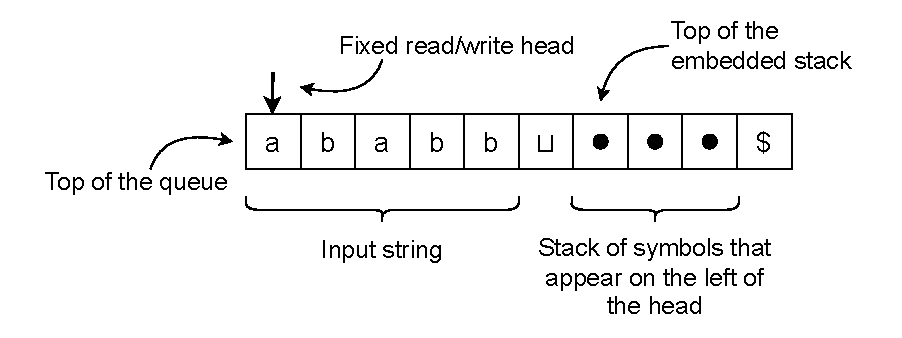
\includegraphics[scale=0.8]{Figures/Problem3.14a.pdf} \\
Organization of the queue.
\end{center}

Define four new operations to manipulate the contents of the queue.
\begin{enumerate}
\item \textit{Rotate-All}. Repeatedly pull and push symbols until the $\$$ is pulled and pushed.
\item \textit{Rotate-Input}. Repeatedly pull and push symbols until the $\#$ is pulled and pushed.
\item \textit{Stash}. Pull a symbol from the queue and place it on top of the embedded stack. To perform a stash, first pull an initial symbol and rotate-input. Then, push the symbol, which was pulled initially and rotate-all.
\item \textit{Restore}. Remove top symbol from the embedded stack and place it on top of the queue. If the embedded stack is empty, then do nothing. Otherwise, first rotate-input, pull a symbol and then rotate-all. Then, push previously pulled symbol and rotate-all.
\end{enumerate}

All the operations of Turing machine tape can be simulated using above operations. To read and write at the current head position, pull from the queue, push the symbol to be written and rotate-all. Stash to move right, and restore to move left. While reading, if $\#$ is pulled, then interpret it as reading a blank. Also, writing happens a bit differently in this case. First, push $\#$ followed by rotate-all, and then push the symbol to be written and rotate-all again.




\begin{center}
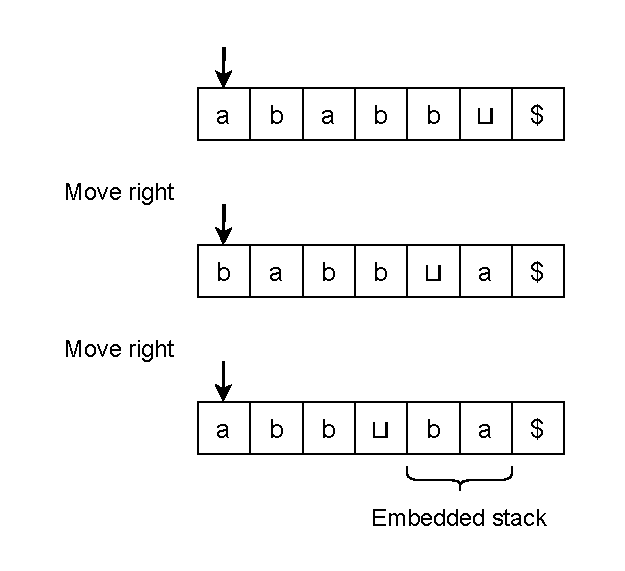
\includegraphics[scale=0.8]{Figures/Problem3.14b.pdf} \\
Simulation of move right.
\end{center}
\end{proof}

\end{document}